\documentclass{acm_proc_article-sp}

% math
\usepackage{amsmath}

% algorithm
\usepackage{algorithmicx}
\usepackage{algorithm}% http://ctan.org/pkg/algorithms
\usepackage[noend]{algpseudocode}% http://ctan.org/pkg/algorithmicx

% table
\usepackage{array}
\makeatletter
\newcommand{\thickhline}{%
    \noalign {\ifnum 0=`}\fi \hrule height 1pt
    \futurelet \reserved@a \@xhline
}
\newcolumntype{"}{@{\hskip\tabcolsep\vrule width 1pt\hskip\tabcolsep}}
\makeatother
\usepackage{dcolumn,multirow}
\usepackage{hhline}

\begin{document}

\title{A Novel Similarity-Search method for Mathematical \\ Content in {\ttlit LaTeX} Markup}

\numberofauthors{2} 
%\author{
%\alignauthor Wei Zhong,\; Hui Fang\\
%       \affaddr{Dept. of Electrical and Computer Engineering}\\
%       \affaddr{University of Delaware}\\
%       \affaddr{Newark, DE USA}\\
%       \email{\{zhongwei, hfang\}@udel.edu}
%}

\maketitle
\begin{abstract}
Mathematical content are widely contained by digital document, but major search engines fail to offer a way to search those structural content effectively, because traditional IR methods are deficient to capture some important aspects of math language. 
We propose a similarity-search method for \LaTeX\ math expressions trying to provide a new idea to better search math content.
Our approach uses an intermediate tree representation to capture structural information of math expression, and based on a previous idea, we index math expressions by tree leaf-root paths. 
A search method to limit search set for possible subexpression isomorphism is provided.
We rank search results by a few intuitive similarity metres from both structural and symbolic points of view. 
Experiment shows these proposed measurements can advance effectiveness with respect to our baseline search method.
\end{abstract}

\category{H.3}{Information Search and Retrieval}{Miscellaneous}
\terms{Algorithms}

\keywords{Mathematical Information Retrieval, Structure Matching}

\section{Introduction}
\label{intro}
Mathematics is frequently used in scientific publications, 
the ability to search in mathematical content can be significantly important as most publications today are digitalized.

However, mathematical language is intrinsically different from general text.
For example, math expressions with identical sets of symbols are not necessarily the same, e.g. $ax+(b+c)$ is not similar to $(a+b)x+c$ in terms of semantic meaning,
further, symbols in different formula can be used interchangeably, e.g. both $a^2+b^2=c^2$ and $x^2+y^2=z^2$ can describe Pythagorean theorem,
these properties make IR models such as \textit{bag of words} model deficient. 
Secondly, symbol frequency in a math equation does not indicate its significance in its context, which also makes popular tf-idf weighting ineffective. 
Although many text-based IR researches are still based on these classical IR methods, they have to unify symbols and normalize math expressions by augmentation to accommodate these problems.
In addition, famous math-aware search engines (e.g. \textit{WolframAlpha}) are mainly focusing on computational evaluation of math expressions, without offering the ability to search similar expressions in related document, 
which can be useful particularly in identifying a math entity or searching an existing proof for an equation.

Given the usefulness of similarity search, and the overhead for traditional IR methods to effectively search mathematical content, 
a new approach to search mathematical expressions by similarity is desired.
But there are certain emerging difficulties in measuring the similarity between mathematical expressions.
For example, math language can be transformed to alternative forms, 
and math expressions with the same evaluated value may also be considered relevant. 
However, we are not going to include these problems into our research domain, we are focusing on measuring mathematical expression similarity just as they are, from two perspective: structural similarity and symbolic similarity.
For structural similarity, we introduce some definitions to describe math expressions structural similarity from substructure isomorphism point of view. 
\textit{Operation tree}~\cite{goodsurvey} is used to represent math expressions with immunity to commutative operands and to better capture structural information of math expressions. 
On top of these, we propose a search method to boolean search structurally relevant expressions and approaches to score structural similarity.
As for symbolic similarity, we label our operation tree to unify the symbols so that we are able to identify the similarity if their symbols are different,
at the same time consider symbolic value, e.g. $E=mc^2$ is considered more meaningful when exact symbols are used rather than just being structurally identical with $y=ax^2$.
On the other hand, we provide an way to rank documents higher if they are \textit{$\alpha$-equivalent} to query.
Because changes of symbols in an expression preserve more syntactic similarity when these changes are made by substitution, e.g. for query $x(1+x)$, expression $a(1+a)$ are considered more relevant than $a(1+b)$. 
We have evaluated our method by comparing to a baseline method with only boolean search, and have also reported our results showing both the efficiency and effectiveness of our method.

\pagebreak
\section{Related Work}
Similarity/boolean search for mathematical content is not a new topic,
conference in this topic is getting increasingly research attention and the proposed systems have progressed considerably~\cite{ov}.
DLMF project from NIST~\cite{Youssef03,Youssef05} and MIaS system~\cite{mias11a,mias11,mias:thesis}, notably, use text-based approaches and utilize existing models to deal with math content on top of existing IR tools (i.e. \textit{Apache Lucene}). 
They are commonly using augmentation and normalization (by ordering the subexpressions) to enumerate and represent all possible sequences of commutative subexpressions or operands.
MWS~\cite{Kohlhase06,Kohlhase0p5} takes an \textit{automatic theorem proving} approach and uses \textit{term indexing} to minimize the cost of unification algorithm which is able to find whether two expressions are equivalent, 
however, their index relies on RAM memory~\cite{Kohlhase0p5} and needs to include all sub-terms of a formula~\cite{Kohlhase06}.
A \textit{symbol layout tree} or \textit{presentation tree}~\cite{symbollayout12,WikiMirs13} is introduced to describe geometric layouts of symbols in a formula. 
\cite{WikiMirs13} uses two templates to parse \LaTeX\ markup with two typical operator terms: explicit ones (``\textbackslash frac", ``\textbackslash sqrt", etc.) and implicit ones (``$+$", ``$\div$", etc.) to form a presentation tree,
then extracts original terms and generalized terms from normalized presentation tree, to provide the flexibility of both fuzzy and exact search.
\cite{symbollayout12} uses symbol layout tree as a kind of substitution tree, while \cite{symbolpairs15,symbolpair15:2} have developed a \textit{symbol pairs} idea to capture relative position information between symbols in an expression,
this idea enables key-value lookup to speed search.
Tree edit distance is adopted by \cite{editdisXML11} in which they try to overcome the bad time complexity of original algorithm by summarizing and using a compromised edit distance algorithm, 
\cite{editdisXML13} improves the speed further by applying an early termination algorithm along with a distance cache.
There are also efforts using image-based approaches~\cite{imageb11,handwrite} and lattice-based approach~\cite{lattice} to measure math formula similarity in a different perspective.

\section{Methodology}
\begin{figure}
\begin{minipage}[b]{1.60in}
\begin{center}
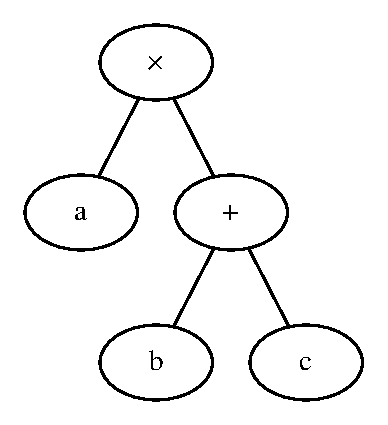
\epsfig{height=1.3in,width=1.0in,file=res/leafroottree.eps}
\\$a(b+c)$ in operation tree
\end{center}
\end{minipage}
\hspace*{0in}
\begin{minipage}[b]{1.60in}
\begin{center}
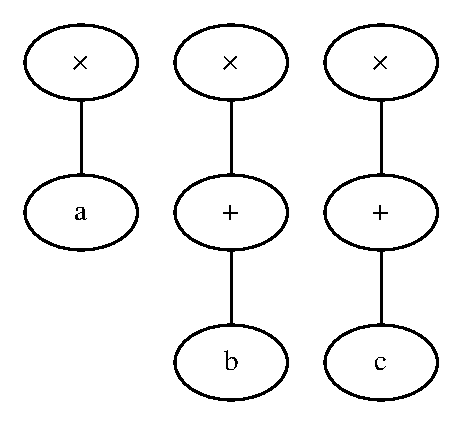
\epsfig{height=1.3in,width=1.2in,file=res/leafrootpath.eps}
Generated leaf-root paths
\end{center}
\end{minipage}
\caption{Leaf-root path example}\label{oprtreeExample}
\end{figure}
Our method can be seen as an approach built upon the idea of leaf-root path or sub-path~\cite{signifjap,MathMLleafroot,signfused,sefobyfo} from an operation tree, to capture structure information of math expression. 
Figure~\ref{oprtreeExample} is an example of generated leaf-root paths for math expression $a(b+c)$.
The intuition behind this idea is that no matter how operands are ordered, an operation tree uniquely determines the leaf-node paths decomposed from the tree.
This makes leaf-root path a good fit for representing mathematical expression because commutative operands are exhaustively used in mathematical language.
Besides, by going bottom-up from leaves of an operation tree, we are essentially traversing to an expression from its subexpression for every level. 
So we can index the leaf-root paths and search an expression by going through and beyond the leaf-root paths from its subexpression.

We develop these ideas to simultaneously search along the way of all leaf-root paths from a given query operation tree, so that we are essentially pruning indexes whose leaf-root paths do not share the common postfixes beyond the root of the query tree.
To better describe this idea and further ideas based upon this, we will put it in a formal way.

\subsection{Formal Definition}
Here we clarify some notations used throughout this paper. 
A \textit{path} $p$ is a sequence of numbers given by $p = p_0 p_1 \ldots p_n$ where $n\ge0$, $p_i \in \mathbf{R}$. $\mathbf{P}$ is the set of all paths.
A \textit{leaf-root path} is a path from root to a leaf in a tree.
Any function $f: \mathbf{R} \rightarrow \mathbf{R}$ applied on path $p$ is mapped to a path too: $f(p)=f(p_0)f(p_1) \ldots f(p_n)$.
And we name  a \textit{concatenation} of two paths $\,^1p = p_0p_1 \ldots p_n$ and $\,^2p = p_np_{n+1} \ldots p_m$ where $m \ge n$, to be a new path denoted as $\,^1p \cdot \,^2p = p_0p_1 \ldots p_n p_{n+1} \ldots p_m$,
and the concatenation of a path $p$ on a path set $S = \{ s_1, s_2 \ldots s_n \}$ is defined as $S \cdot p = \{ s_1\cdot p,\  s_2\cdot p \ \ldots \ s_n\cdot p \}$.
The \textit{longest common prefix} path $p^*$ between two paths $p_1$ and $p_2$ is mapped by the function named $\mathrm{lcp}$, which is defined by $p^* = \mathrm{lcp}(p_1, p_2) = \mathrm{lcp}(p_2, p_1)$.

We introduce a \textit{formula tree} to represent a mathematical expression, in which each node is associated with a label to represent an unified token (e.g. same value for token $+$, $\oplus$ and $\pm$) and each leaf node is associated with a number to identify original operand symbol. 
Besides, a \textit{formula subtree} relation is also defined to address the sub-structure relation between two mathematical expressions.

\subsubsection{Formula tree}
A \textit{formula tree} is a labeled rooted tree $T = T(V,E,r)$ with root $r$, where each vertices $v \in V(T)$ is associated with a label (not necessarily unique in the same tree) $\ell_T(v) \in \mathbf{R}$ mapped by label function $\ell_T$,
and each leaf $l \in V(T)$ is further associated with a symbol $\mathcal{S}_T(l) \in \mathbf{R}$ mapped by symbol function $\mathcal{S}_T$. 
For convenience, we will write function $\ell$ and $\mathcal{S}$ as their short names which refer to the tree implied by the context, and we use $\mathcal{S}(p)$ to indicate the symbol of the leaf in a leaf-root path $p$.
In addition, we use $^s T$ to denote a subtree in $T$ rooted by vertices $s \in V(T)$, with all its descendants.

\subsubsection{Formula subtree}
\label{frmlsubtreeDef}
Given formula tree $S$ and $T$, we say $S$ is a \textit{formula subtree} of $T$ if there exists an injective mapping $\phi: V(S) \rightarrow V(T)$ satisfying:

\begin{enumerate}
\item 
$\forall\; (v_1,v_2) \in E(S)$, we have $(\phi(v_1),\phi(v_2)) \in E(T)$;
\item
$\forall\; v \in V(S)$, we have $\ell(v) = \ell(\phi(v))$;
\item
If $v \in V(S)$ is a leaf vertices in $S$, then $\phi(v)$ is also a leaf in $T$.
\end{enumerate}
Such a mapping $\phi$ is called a \textit{formula subtree isomorphic embedding} (or \textit{formula embedding}) for $S \rightarrow T$. 
If satisfied, we denote $S \preceq_l T$ on $\Phi$, where $\Phi$ ($\Phi \neq \emptyset$) is the set of all the possible formula embeddings for $S \rightarrow T$.

\subsubsection{Leaf-root path set}
A \textit{leaf-root path set} generated by tree $T$ is a set of all the leaf-root paths from tree $T$, mapped by a function $g(T)$. 

\subsubsection{Index}
An \textit{index} $\Pi$ is a set of trees such that $\forall\; T \in \Pi$, we have $T \in \mathcal{I}_{\Pi}(a)$ for any $a \in \ell(g(T))$, we say $T$ is \textit{indexed} in $\Pi$ and $\mathcal{I}_{\Pi}$ is called \textit{index look-up function} for index $\Pi$. 

\subsection{Search Method}
\label{se-method}
For a collection of document expressions, we will index them by merging all the reverted leaf-root paths from each document formula tree into a large ``inverted" index tree, 
in which each node at path $a$ stores the information of all the indexed formula trees in $\mathcal{I}_{\Pi}(a)$.

Through searching all sub-paths from a query formula tree $T_q$ at the same time, we are able to limit the set of possible formula trees being structurally matching (in formula subtree relation) with $T_q$, to only a subset of our index. 
This is illustrated as follows.

Given an index $\Pi$ and a formula tree $T_q$, $\forall\; T_d \in \Pi$:
If $T_q \preceq_l T_d$ on $\Phi$, then $\exists\; \hat{a} \in \mathbf{P},\; s.t.$
$$
T_d \in \bigcap_{a \in L} \mathcal{I}_{\Pi}(a)
$$
where $L = \ell(g(T_q)) \cdot \hat{a}$.

\textit{Justification.}
Denote the root of $T_q$ and $T_d$ as $r$ and $s$ respectively.
Let $\hat{p}$ be the path determined by vertices from $t=\phi(r)$ to $s$ in $T_d$,
and $\,^1p, \,^2p \ldots \,^np,\; n \ge 1$ be all the leaf-node paths in $T_q$.
Then $\hat{a} = \ell(\hat{p})$, this is because:
$L = \ell(\{ \,^1p, \,^2p \ldots \,^np \}) \cdot \hat{a} = 
\ell(\{ \phi(\,^1p), \phi(\,^2p) \ldots \phi(\,^np) \}) \cdot \ell(\hat{p}) =
\{ \ell(\phi(\,^1p) \cdot \hat{p}), \ell(\phi(\,^2p) \cdot \hat{p}) \ldots \ell(\phi(\,^np) \cdot \hat{p}) \}
$.
According to definition~\ref{frmlsubtreeDef} and $t=\phi(r)$, we have $\phi(\,^ip) \cdot \hat{p} \in g(T_d),\; 1 \le i \le n$.
Since $ T_d \in \Pi$, $T_d$ is indexed in $\Pi$ with respect to each of the elements in $L$, that is to say $\forall\; a \in L, \; T_d \in \mathcal{I}_{\Pi}(a)$.

\begin{figure}
\begin{minipage}[b]{1.65in}
\begin{center}
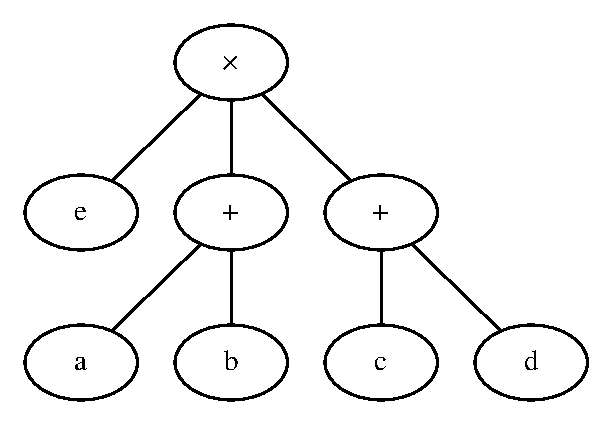
\epsfig{height=1.3in,width=1.6in,file=res/not-necessary.eps}
\\ $(a+b) \times (c+d) \times e$
\end{center}
\end{minipage}
\hspace*{.0in}
\begin{minipage}[b]{1.60in}
\begin{center}
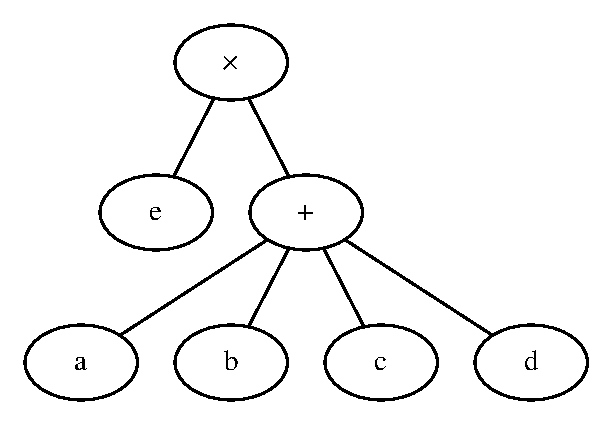
\epsfig{height=1.3in,width=1.5in,file=res/not-necessary2.eps}
\\ $(a+b+c+d) \times e$
\end{center}
\end{minipage}
\caption{Leaf-root paths with different structure}\label{notnecessary}
\end{figure}

In a nutshell, we search the index by intersecting the indexed formula trees from all the generated leaf-node paths at the same time, then further possible search path $\hat{a}$ is only possible when paths along the generated leaf-node paths in the index have a common postfix.
Therefore we can ``merge" the paths ahead and prune those paths not in common. Level by level, we are always able to find the structurally matched formula tree as long as it is indexed in $\Pi$.

\subsection{Substructure Matching}
However, query formula tree will not necessarily be formula subtree of all the document (indexed) formula trees in our search set
$\bigcap_{a \in L} \mathcal{I}_{\Pi}(a)$,
even if their generated leaf-root paths are identical.
One supporting example for this point is shown in figure~\ref{notnecessary}.
To address this problem, we propose an algorithm described in in figure~\ref{submatchalgo}, to test the document formula trees in our search set to see if they are in formula subtree relation with query formula tree.
This algorithm is inspired from the following observations. 

\begin{figure}
\begin{algorithmic}[1]

\Procedure{removeCandidate}{$d,Q,C$}
\For {$a \in Q$}
\If{$C_a = \emptyset$}
\State \textbf{return} $\emptyset$
\Else
\State {$C_a := C_a - \{d\}$}
\EndIf
\EndFor
\State \textbf{return} $C$
\EndProcedure

\State {}

\Procedure{match}{$a, a', Q, C$}
\For {$b \in Q$}
\State $t := \big| \mathrm{lcp}(a,b) \big|$
\State $Q_t := Q_t \cup \{b\}$
\State $P := P \cup \{t\}$
\EndFor
\For {$t \in P$}
\For {$b \in Q_t$}
\For {$b' \in C_b$}
\If {$t \not= \big| \mathrm{lcp}(a',b') \big|$}
\State $C := $ \Call{removeCandidate}{$b', Q_t, C$}
\If {$|C| = 0$}
\State \textbf{return} FAIL
\EndIf
\EndIf
\EndFor
\EndFor
\If {\Call{decomposeAndMatch}{$Q_t, C$} = FAIL}
\State \textbf{return} FAIL
\EndIf
\EndFor
\State \textbf{return} SUCC
\EndProcedure

\State {}

\Procedure{decomposeAndMatch}{$Q, C$}
\If {$Q = \emptyset$} \textbf{return} SUCC
\EndIf
\State $a$ := OnePathIn(Q)
\Comment{Choose a reference path in Q}
\State $Q_{\mathrm{new}} := Q - \{a\}$
\For {$a' \in C_a$}
\State $C_{\mathrm{new}} := $ \Call{removeCandidate}{$a', Q_{\mathrm{new}}, C$}
\If {$C_{\mathrm{new}} = \emptyset$} \textbf{return} FAIL
\EndIf
\If {\Call{match}{$a, a', Q_{\mathrm{new}}, C_{\mathrm{new}}$}}
\textbf{return} SUCC
\EndIf
\EndFor
\State \textbf{return} FAIL
\EndProcedure

\end{algorithmic}
\caption{The decompose-and-match algorithm}\label{submatchalgo}
\end{figure}

\subsubsection{Observation 1} 
\label{observation1}
For two formula trees which satisfy $T_q \preceq_l T_d$ on $\Phi$, then $\forall\; \phi \in \Phi,\, p \in g(T_q)$, also any vertices $v$ along path $p$, the following properties are obtained:
\begin{eqnarray}
\deg(v) \le \deg(\phi(v)) \label{prop1} \\
\ell(p) = \ell(\phi(p)) \label{prop3} \\
\left| g(T_q) \right| \le \left| g(T_d) \right| \label{prop4}
\end{eqnarray}
\textit{Justification.} 
Because $\forall\; w \in V(T_q) \  s.t. \  (v, w) \in E(T_q)$, there exists $(\phi(v), \phi(w)) \in E(T_d)$. 
And for any (if exists) two different edges $(v, w_1), (v, w_2) \in E(T_q),\, w_1 \not= w_2 \in V(T_q) $, we know $(\phi(v), \phi(w_1)) \not= (\phi(v), \phi(w_2))$ by definition~\ref{frmlsubtreeDef}. 
Therefore any different edge from $v$ is associated with a distinct edge from $\phi(v)$, thus we can get (\ref{prop1}). 
Given the fact that every non-empty path $p$ can be decomposed into a series of edges $(p_0, p_1), (p_1, p_2) \ldots (p_{n-1}, p_n), \; n > 0$,
property (\ref{prop3}) is trivial.
Because there is exact one path between every two nodes in a tree, the leaf-root path is uniquely determined by a leaf node in a tree. Hence the rationale of (\ref{prop4}) can be obtained in a similar manner with that of (\ref{prop1}), expect neighbor edges are replaced by leaf-node paths.


\subsubsection{Observation 2} 
\label{observation2}
Given two formula trees $T_q$ and $T_d$, if $\left| g(T_q) \right| = 1$ and $\ell(g(T_{q})) \subseteq \ell(g(T_d))$, then $T_q \preceq_l T_d$.

\noindent \textit{Justification.} 
Obviously there is only one leaf-root path in $T_q$ because $\left| g(T_q) \right| = 1$. 
Denote the path as $p = p_0 \ldots p_n,\; n \ge 0$ where $p_n$ is the leaf.
Since $\ell(p) \subseteq \ell(g(T_d))$, we know that there must exist a path $p'=p'_0 \ldots p'_n \in g(T_d)$ such that $\ell(p) = \ell(p')$ 
where $p'_n$ is the leaf of $T_d$.
%Without loss of generality,  
Then
the injective function $\phi: p_i \rightarrow p'_i,\  0 \le i \le n$ satisfies all the requirements for $T_q$ as a formula subtree of $T_d$.

\subsubsection{Observation 3} 
\label{observation3}
For two formula trees $T_q$ and $T_d$, if $T_q = T(V,E,r) \preceq_l T_d$ on $\Phi$,  
$\forall a,b \in g(T_q)$ and a mapping $\phi \in \Phi$. 
Let $T_d' = \, ^{t}T_d$ where $t = \phi(r)$ and $a' = \phi(a)$, $\forall\; b' \in g(T_d')$, it follows that:
$$
\begin{array}{lcr}
b' = \phi(b)  & \Rightarrow & 
\left| \mathrm{lcp}(a,b) \right| = \left| \mathrm{lcp}(a',b') \right|
\end{array}
$$
Furthermore, $\forall\; c \in g(T_q)\; s.t.\; \left| \mathrm{lcp}(a,b) \right| \neq \left| \mathrm{lcp}(a,c) \right| $, we have
$$
\begin{array}{lcr}
\left| \mathrm{lcp}(a,b) \right| = \left| \mathrm{lcp}(a',b') \right|
& \Rightarrow &
b' \neq \phi(c)
\end{array} 
$$
\textit{Justification.} 
Because $a,b \in g(T_q)$, thus $a_0 = b_0 = r$, and we can also make sure $\mathrm{lcp}(a,b) \ge 1$. 
Denote the path of $a = a_0 \ldots a_n a_{n+1} \ldots a_{l-1}$, similarly denote the path of $b$ as $b=b_0 \ldots b_n b_{n+1} \ldots b_{m-1}$,
where the length of each $l,m \ge 1$ and $a_i = b_i,\, 0 \le i \le n \le \min(l-1, m-1)$ while $a_{n+1} \neq b_{n+1}$ if $l,m > 1$.
On the other hand $a' = \phi(a)$ and $b' \in g(\,^{t}T_d)$, therefore $a'_0 = \phi(a_0) = \phi(r) = t = b'_0$.
For the first conclusion, if $b' = \phi(b)$, there are two cases. If either $|a|$ or $|b|$ is equal to one then $\left| \mathrm{lcp}(a,b) \right| = \left| \mathrm{lcp}(a',b') \right| = 1$;
Otherwise if $l,m > 1$, path $a_0 \ldots a_n = b_0 \ldots b_n$ and $a_{n+1} \neq b_{n+1}$ follow that $\phi(a_0 \ldots a_n) = \phi(b_0 \ldots b_n)$ and $\phi(a_{n+1}) \neq \phi(b_{n+1})$ by definition.
Because edge $(\phi(a_n), \phi(a_{n+1}))$ and $(\phi(b_n), \phi(b_{n+1}))$ are both in $E(T'_d)$, 
we have $\left| \mathrm{lcp}(a,b) \right| = \left| \mathrm{lcp}(a',b') \right| = n$.
For the second conclusion, we prove by contradiction. 
Assume $b' = \phi(c)$, by the first conclusion we know $\left| \mathrm{lcp}(a,c) \right| = \left| \mathrm{lcp}(a',b') \right|$.
On the other hand, because $\left| \mathrm{lcp}(a,c) \right| \neq \left| \mathrm{lcp}(a,b) \right| =  \left| \mathrm{lcp}(a',b') \right|$, 
thus $\left| \mathrm{lcp}(a,c) \right| \neq \left| \mathrm{lcp}(a',b') \right|$ which is impossible. 

For a query formula tree $T_q$ and a document formula tree $T_d$, observation 1 offers us some constrains for finding initial possible isomorphic paths in $T_d$ (what we call \textit{candidates}) for a given query path in $T_q$.
Observation 2 is a sufficient condition to test substructure relation, however, the query tree has to have only one leaf-root path to be tested. 
And observation 3 states two necessary conditions for one formula tree to be a formula subtree of another and implies that a group of query leaf-root paths can only be isomorphic to someones in another group of leaf-root paths in document formula tree. 
This leads to the idea to decompose the formula tree and divide the problem into subproblems by ruling out impossible candidates using observation 3, until at some point we can apply observation 2 or observe trivial cases to solve all the sub-matching problems.

\begin{figure}
\begin{minipage}[b]{1.65in}
\begin{center}
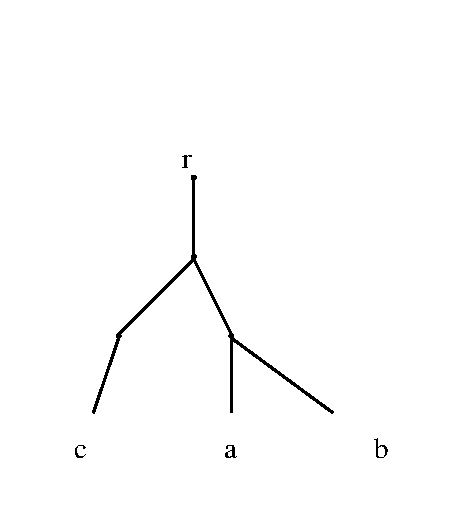
\epsfig{height=1.9in,width=1.6in,file=res/lpd.eps}
\\(a)
\end{center}
\end{minipage}
\hspace*{0in}
\begin{minipage}[b]{1.65in}
\begin{center}
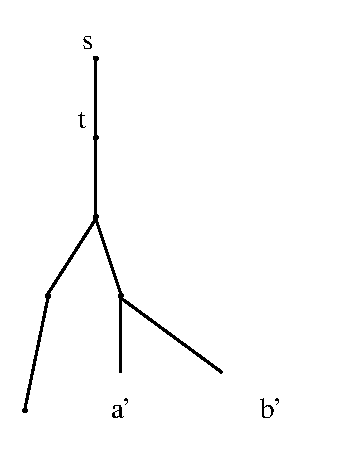
\epsfig{height=1.9in,width=1.6in,file=res/lpd2.eps}
\\(b)
\end{center}
\end{minipage}
\caption{Formula subtree matching}\label{submatch}
\end{figure}

To illustrate our \textproc{decomposeAndMatch} algorithm, figure~\ref{submatch} gives a general case in which query tree in (a) is trying to match a document tree in (b).
Initially every leaf-root path in (a) should be associated with a set of candidate paths in (b) which satisfy the constrains in \ref{observation1}.
Then we arbitrarily choose a path in (a) as a \textit{reference path} (heuristically a \textit{heavy path}~\cite{heavypathde}), for each of the paths in its candidate set, we choose it as reference path in (b), and suppose we choose $a'$ here. At this time we can apply the two constrains from \ref{observation3} and ruling out some impossible isomorphic paths in candidate set of each path in (a) and divide the problems further. 
For example, because $\left| \mathrm{lcp}(a,b) \right| = \left| \mathrm{lcp}(a',b') \right|$, we know $b'$ is still in candidate set of $b\,$; while $b'$ is not in candidate of $c$ because $\left| \mathrm{lcp}(a,b) \right| \neq \left| \mathrm{lcp}(a,c) \right|$. 
After going through these eliminations for each leaf-node path (except the reference path $a$) in (a), we now have two similar subproblems: $c$ as a subtree along with its candidate set, and $b$ as a subtree along with its candidate set. 
We can apply this algorithm recursively until a trivial subproblem is reached (e.g. the case in \ref{observation2}). During this process, if we find any candidate set to be empty, we stop the subproblem process and change to another reference path or stop the algorithm completely if every possible reference path is tried.
The argument $Q$ and $C$ is the set of leaf-root paths in query tree and the candidate sets associated with all query tree leaf-root paths respectively.
The procedure returns \textproc{SUCC} if a matching possibility is found, otherwise \textproc{FAIL} is returned indicating the formula tree in (a) cannot be a formula subtree of that in (b).

\textproc{decomposeAndMatch} algorithm offers a way to ``double-check" structure isomorphism, because 
for any two formula tree $T_q$ and $T_d$ and $\forall\; \hat{a} \in \mathbf{P}$, if $\ell(g(T_q)) \cdot \hat{a} \subseteq \ell(g(T_d))$, it is not sufficient to imply $T_q \preceq_l T_d$.
Nevertheless, we think the cases which makes the above statement insufficient are fairly rare in common mathematical content, and the complexity introduced from this algorithm will offset the benefit to identify the structure isomorphism.
Thus a compromised search, for efficiency reason, would assume all the document formula trees in search set
$\bigcap_{a \in L} \mathcal{I}_{\Pi}(a)$ is structurally matching the given query formula tree $T_q$.

\subsection{Structural Similarity}
After searching structurally matched document expressions in a boolean manner, we use two factors to measure their structural similarity degree. 

The first factor is \textit{matching depth}.
As it is addressed in \cite{mias11a}, the deeper sub-formulae in in mathematical expression will make it less important to the overall formula.
For example, given query formula $\sqrt a$, expression $\sqrt {x}$ would score higher than $\sqrt{\sqrt{x}}$ does. 
To reflect the depth where two expressions match, we define \textit{matching depth factor} $f(d)$ to be a function value in negative correlation with matching depth $d = |\hat{a}|$, e.g. $f(d) = 1/(1 + d)$ in our method.
The second factor is \textit{matching ratio}. According to the property $(3)$ in \ref{observation1}, 
we have $|g(T_q)| / |g(T_d)| \le 1$, and the ratio on the left-hand is defined as \textit{matching-ratio}, which characterises the structural coverage for the matching part in an expression.
Intuition behind this is, for example, given query $\alpha y + \beta$, document expression $ax + b$ should precede $x^2 + ax + b$ simply because the query matches more ``area" of the former expression than that of the latter.

\subsection{Symbolic Similarity}
As we have discussed in section~\ref{intro}, besides structural similarity, symbolic similarity is also essential to be considered.
Here our scoring goal for symbolic similarity can be summarized in two points:
\begin{itemize}
\item Given two formula trees
$T_q \preceq_l T_d$ on $\Phi$,  
suppose a leaf $l \in V(T_q)$ is isomorphic to leaf $l' \in V(T_d)$, that is to say, $\phi(l)=l'$, where $\phi \in \Phi$, then if their symbol matches, i.e. $\mathcal{S}(l) = \mathcal{S}(l')$, we score them higher than those do not match symbolically. And the more symbolic matches there are, the higher symbolic relevance degree two expressions have.
\item $\alpha$-equivalent expressions have more symbolic relevance degree than those are not, and the more \textit{bond variables} (those with same symbol in an expression) two expressions match at the structurally matching positions, the more symbolically relevant they are considered to be.
\end{itemize}

The two are illustrated as follows. 
Let the rank of a structurally relevant document expression $d$ be $r(d)$, and given query $\sqrt a (a - b)$ for instance. 
Then the first goal is essentially saying 
$$
r\big(\sqrt a (a - b)\big) > r\big(\sqrt a (a - y)\big) > r\big(\sqrt x (x - y)\big)
$$
because here the second document has two symbols matching while the third document has no symbolic match at all. 

By the second goal, we know
$$
r\big(\sqrt x (x - b)\big) > r\big(\sqrt x (y - b)\big)
$$
in which the second document does not have a bond-variable match as the first document does with the query.

However, sometimes the two goals can be conflicting.
Given document expression $\sqrt a (x - b)$ and $\sqrt x (x - b)$ for instance, the former has two symbolic matches (i.e. ``$a$" and ``$b$") while it does not have bond-variable match. On the other hand, the latter has bond-variable match while it only has one symbolic match (i.e. ``$b$"). 
We nevertheless score the latter higher because it does not lose any mathematic semantics. 

\begin{figure}
\begin{algorithmic}[1]

\Procedure{markAndCross}{$D,Q,C$} 
\State score := 0

\If {$D = \emptyset$} 
\State \textbf{return} 0 
\EndIf
\For {$a' \in D$}
\State $T_{a'} := \mathrm{unmark}$ 
\EndFor
\For {$v \in \mathcal{V}(D)$}
\State $B_v := 0$ 
\EndFor

\State QList := \Call{sortByOccurAndSymbol}{Q}

\For {$a$ {\bf in} QList}

\For {$v \in \mathcal{V}(D)$}
\State $m := -\infty$
\State $m_p := \varnothing$
\For {$a' \in C_a \cap \{ y \mid \mathcal{S}(y) = v,\ y \in D\} $}
\If {$T_{a'} = \mathrm{unmark}$ {\bf and} $\mathrm{sim}(a, a') > m$} 
\State $m := \mathrm{sim}(a, a')$ 
\State $m_p := a'$ 
\EndIf
\EndFor
\If {$m_p \not= \varnothing$}
\State $T_{m_p} := \mathrm{mark}$ 
\State $B_v := B_v + m$
\Else
\Comment{Exhausted all candidates}
\State \textbf{return} 0 
\EndIf
\EndFor

\If {$\mathcal{S}(a) \mathrm{\ changed}$ {\bf or} $\mathrm{\ last\ iteration\ of\ } a$}
\label{line_bond_finish}

\State $m := -\infty$
\State $m_v := \varnothing $
\For {$v \in \mathcal{V}(D)$}
\If {$B_v > m$} 
\State $m := B_v$ 
\State $m_v := v$ 
\EndIf
\State $B_v := 0$ 
\EndFor
\State $\mathrm{score} := \mathrm{score} + m$ 

\For {$v \in \mathcal{V}(D)$}
\If {$v = m_v$} 
\State $\mathrm{nextState} := \mathrm{unmark}$ 
\Else
\State $\mathrm{nextState} := \mathrm{cross}$ 
\EndIf
\For {$a' \in C_a \cap \{ y \mid \mathcal{S}(y) = v,\ y \in D\} $}
\If {$T_{a'} = \mathrm{mark}$} 
\State $T_{a'} := \mathrm{nextState}$ 
\EndIf
\EndFor
\EndFor

\EndIf

\EndFor

\State \textbf{return} score
\EndProcedure

\end{algorithmic}
\caption{The mark-and-cross algorithm}\label{markcrossalgo}
\end{figure}

To meet the goals above, intuitively, we first take the bond variable with greatest number of occurrence in query expression, try to match as much as possible with each bond variable from document expression. 
The \textit{best-matching} bond variable in document expression is chosen to contribute to the final symbolic relevance score (proportionally to the number of matches in that bond variable), 
and we exclude its paths from matching query paths in future iterations.
In the next iteration, we choose the bond variable with the second number of occurrence in query expression and repeat this process until all the query bond variables are iterated.

We describe our algorithm in figure~\ref{markcrossalgo} which measures symbolic similarity given two expressions. 
The \textproc{markAndCross} algorithm takes 
three arguments, the set of leaf-root paths $D$ and $Q$ in document expression and query expression respectively, and the candidate sets $C$ associated with all leaf-root paths in query. 
The bond variables in $D$ is addressed by the set $\mathcal{V}(D) = \{x \mid \mathcal{S}(x),\ x \in D\}$, which contains all the leaf node symbols from document expression.
Procedure \textproc{sortByOccurAndSymbol} takes a set of leaf-root paths and returns a list containing all the paths. 
The list is sorted by tuple $\big(N_p, \mathcal{S}(p)\big)$ for list element $p$, where $N_p$ is the number of $\mathcal{S}(p)$ occured in all the list path symbols. 
Each document path $a'$ is associated with a tag $T_{a'}$ which has three possible states: marked, unmarked and crossed. And bond variable $v \in \mathcal{V}(D)$ can be given a score $B_v$ which represents the similarity degree between current evaluating query/document bond variables. 
The function $\mathrm{sim}(a,a')$ measures the symbolic similarity degree between two leaf-root paths $a$ and $a'$. 
Intuitively, we set the similarity function
$$
\mathrm{sim}(a,a') = 
\left\{
\begin{array}{ll}
1    &\qquad \mathrm{if}\  \mathcal{S}(a) = \mathcal{S}(a')
\\
\\
\alpha < 1  &\qquad \mathrm{otherwise}
\end{array}
\right.
$$
to give more similarity weights to leaf-root paths with exact symbol match.

Let us determine the proper value for $\alpha$. 
Consider the conflicting cases stated in this section by using another example here, 
given query expression $a+\frac 1 a + \sqrt{a}$ and document expression $a+\frac 1 a + b + \frac 1 b + \sqrt{b}$, we consider bond-variable matching 
$$\fbox{a}+\dfrac 1 {\fbox{a}} + \sqrt{\fbox{a}}$$
with 
$$a+\dfrac 1 a + \fbox{b} + \dfrac 1 {\fbox{b}} + \sqrt{\fbox{b}}$$
weighted more than exact symbol matching 
$$\fbox{a}+\dfrac 1 {\fbox{a}} + \sqrt{a}$$ 
with 
$$\fbox{a}+\dfrac 1 {\fbox{a}} + b + \dfrac 1 b + \sqrt{b}$$
(expressions surrounded by a box here indicates the matching part)

Because the former matching has more variables involved even if they are not identical symbolic matches compared with its counterpart of the latter. 
That is to say, given a document bond-variable matching $k$ variables with that in query, we need $\alpha$ to satisfy $ k \alpha > (k-1) \times 1 = k - 1 $
and $\alpha < 1$. 
Therefore, in our practice, we set $\alpha$ to a value close to $1$, e.g. $0.9$.

By sorting the query paths in $Q$, the algorithm is able to take out paths from same bond variable in maximum-occurrence-first order from QList. 
Each query path $a$ tries to match a path $a'$ in each document bond variable $v$ by selecting the unmarked path $m_p$ with maximum $\mathrm{sim}(a,a')$ value, and accumulate this value on $B_v$ indicating the similarity between currently evaluating query bond variable and the bond variable $v$ in document expression.
In addition, mark the tag $T_{m_p}$ associated with the document path $m_p$.
Once a query bond variable has been iterated completely (line~\ref{line_bond_finish}),
let the document bond variable $m_v$ with greatest $B_v$ value $m$, be the best-matching bond variable in $\mathcal{V}(D)$ with the query bond variable just iterated, then add $m$ to the score.
Before iterating a new query bond variable, we will cross all the document paths of variable $m_v$ to indicate they are confirmed been matched, 
and unmark the tags of those marked paths that are not variable $m_v$.
We continue doing so until all the query paths are iterated, finally return the score indicating the symbolic similarity between the two expressions.

\section{Implementation}
In order to evaluate the performance of our method, we have implemented a proof-of-concept search engine~\footnote{demo page: [link not revealed here for anonymity]} as well as a parser for parsing \LaTeX\ markup content directly into our defined operation trees.

\subsection{Parser}
We are tokenizing math content using lexer generator \textit{flex} and have implemented a LALR parser generated from a set of grammar rules in \textit{GNU bison}, specifically for MathJax content in a subset of \LaTeX\ (those related to mathematics).
Our parser transforms a math formula into an in-memory operation tree (representing formula tree), as an intermediate step to extract the path labels, path ID, and degree numbers associated, for every leaf-root path from the tree. 
Our lexer omits all \LaTeX\ control sequences not matching any pattern of our defined tokens, most of them are considered unrelated to math formula semantics (environment statement, color, mbox etc.).

\subsection{Index}
The indexer writes the information extracted from parser into disk. 
There are two parts in our index, the first part uses native file system (for the sake of implementation simplicity) to store leaf-root path labels in directories from which our search engine can go level by level. 
Path ID, degree numbers, and also the formula ID generating that leaf-root path (we refer these three as \textit{branch word}) are stored in a ``posting" file at the directory corresponding to that branch word labels, 
e.g. the tree in figure~\ref{oprtreeExample} will result in indexing two directories: ./VAR/TIMES and ./VAR/ADD/TIMES. 
All the indexed branch words with path labels corresponding to directory ./VAR/TIMES/ are stored in the posting file of that directory, located at ./VAR/TIMES/posting.bin in this case.
Branch words in a posting file are ordered by their formula IDs to speed merge search.
The second part of our index is a key-value database (using \textit{Kyoto Cabinet}) to map a formula ID to additional information for that formula (e.g. original markup, number of leaf-root paths $|T_d|$ and the URL on which the formula is crawled).

\begin{figure*}
\begin{minipage}[b]{3.40in}
\begin{center}
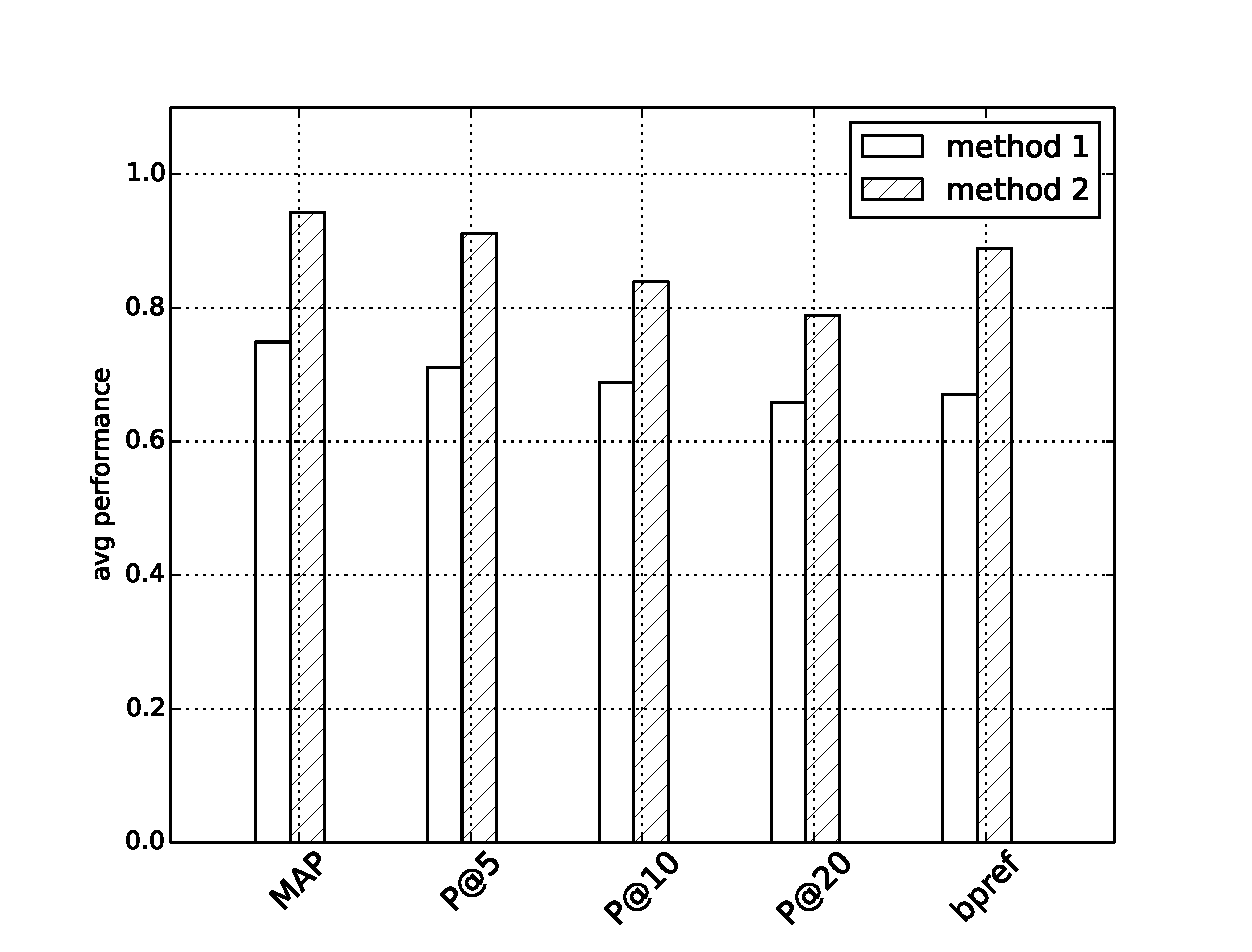
\epsfig{height=2.5in,width=3.4in,file=res/partial-rel.eps}
\\Partial relevance (relevance score $\ge 1$) 
\end{center}
\end{minipage}
\hspace*{0in}
\begin{minipage}[b]{3.40in}
\begin{center}
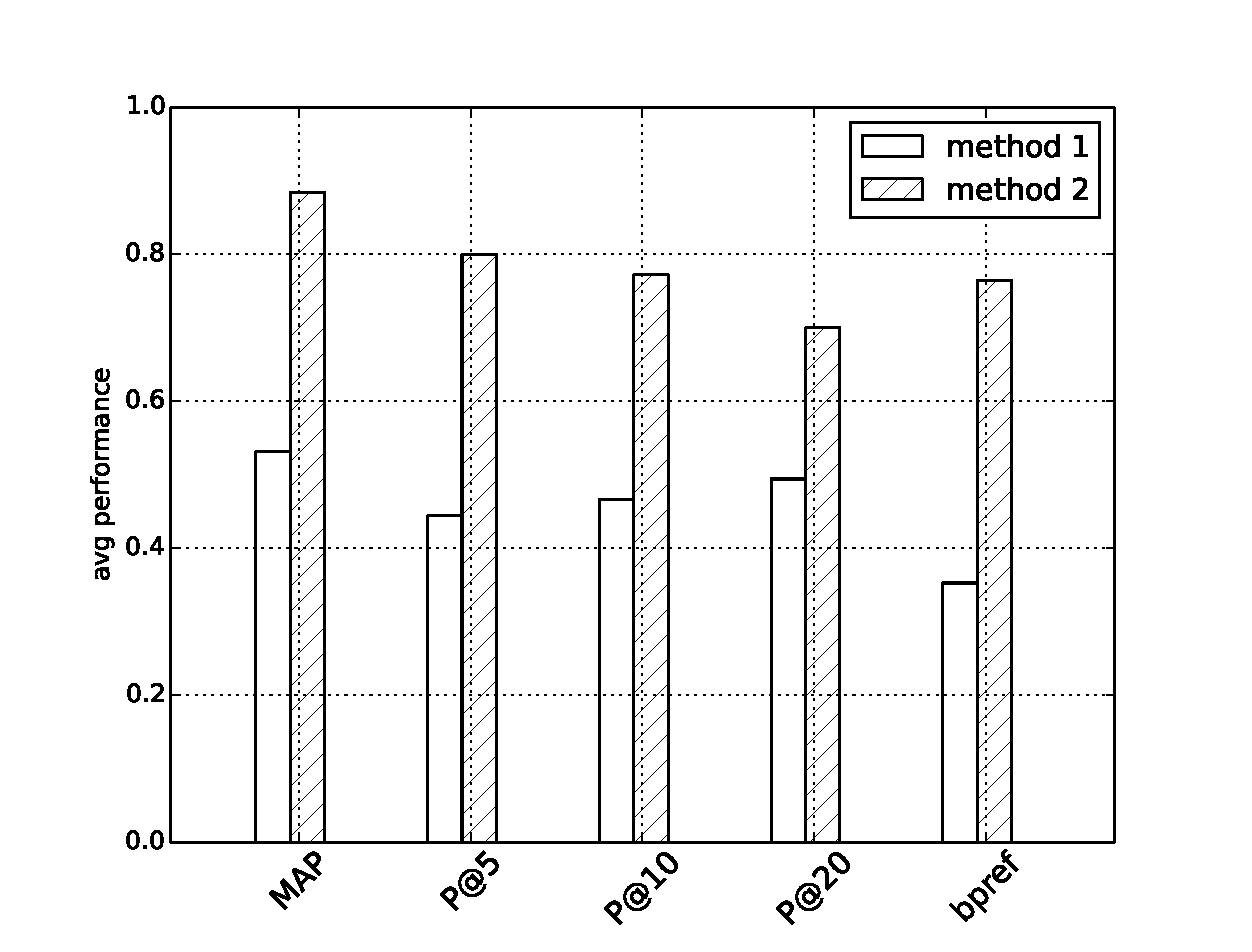
\epsfig{height=2.5in,width=3.4in,file=res/total-rel.eps}
\\Relevance (relevance score $\ge 3$)
\end{center}
\end{minipage}
\caption{Effectiveness performance}\label{perfcomp}
\end{figure*}

\subsection{Searching and Ranking}
\label{se-and-rank}
The compromised substructure searching (described in section~\ref{se-method}) is used in our search engine to filter out likely isomorphic expressions in our index.
Searching is performed by simultaneously going from all the directories corresponding to the generated leaf-root paths of query formula tree,
to all their merged subdirectories. 
We keep traversing, at each level intersect the branch words (by their formula IDs) in the posting files from all the searching directories. 
The intersected formula IDs actually represent the trees in our search set $\bigcap_{a \in L} \mathcal{I}_{\Pi}(a)$.
Every document formula spotted in the search set is considered as a hit, we then apply \textproc{markAndCross} algorithm to get its symbolic similarity score with query formula. 
Denote this score to be $s$, and $f(d)$ being the matching depth factor, $r$ being the matching ratio for a pair of query/document. 
We will use them together in a tuple $(s, f(d), r)$, to indicate the overall similarity and rank items in search results,
i.e. to decide whether one should be ranked higher than the other, first compare $s$, if equal, compare $f(d)$ and then $r$.
In addition, we use a min-heap to keep the top-$k$ scored items in our search results (by replacing the lowest scored items if we find a newer hit with higher score), where $k$ is the maximum number of items we keep in search results.
We also place a valve on the number of branch words can be searched for one query at a time,
so that when exceeding this limit, search engine will stop and return the search results it has up to that time. Because some query can potentially have a very long posting list, doing so would make our searching response time no more than a certain value.

\begin{figure}
\begin{center}
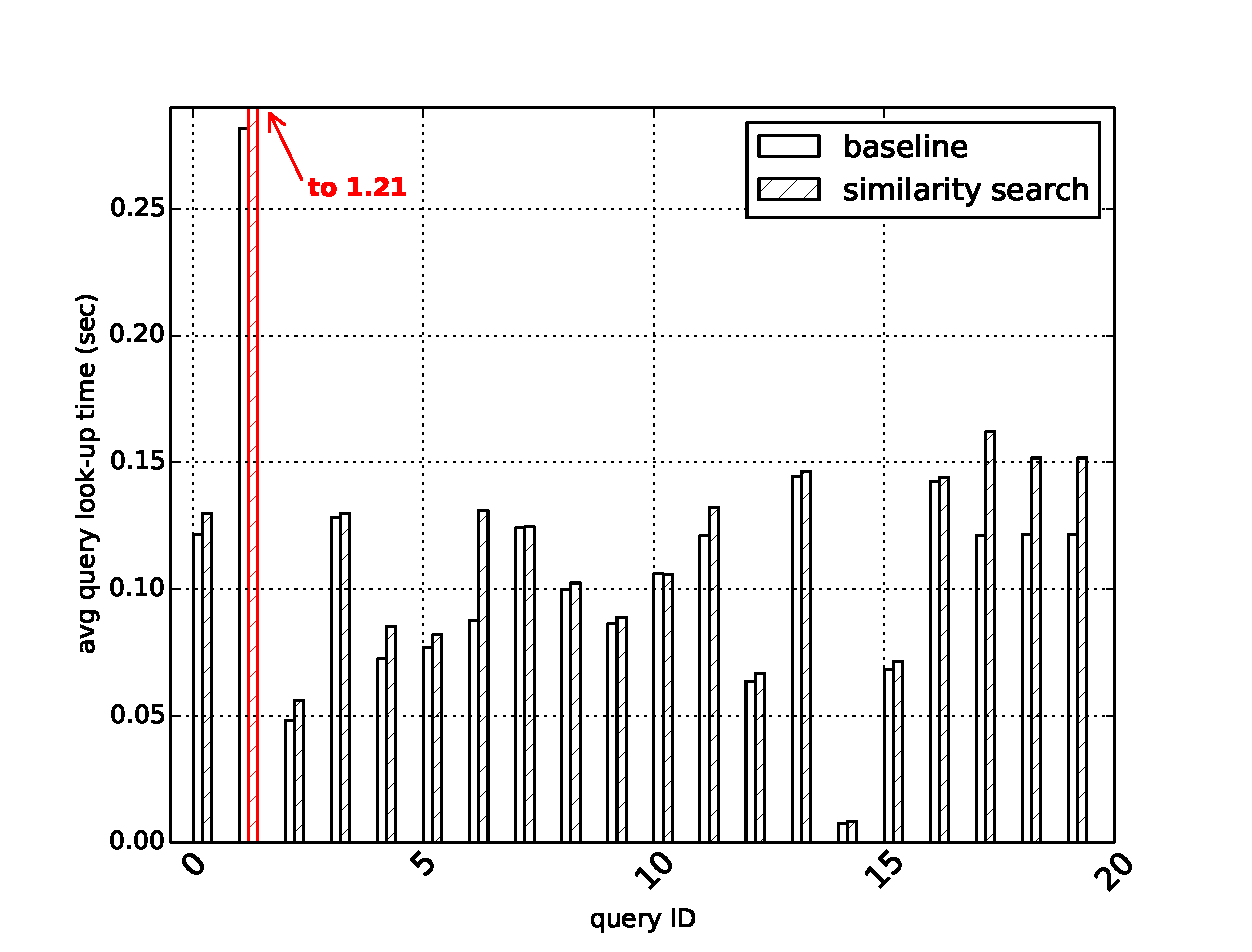
\epsfig{height=2.5in,width=3.55in,file=res/response-time.eps}
\end{center}
\caption{Efficiency performance}\label{effiperf}
\end{figure}

\section{Evaluation}
Our own dataset is created to evaluate proposed method.
We have crawled \LaTeX\ content from the posts of nearly entire (27180 pages of questions) Math Stack Exchange website before March 2015. 
The data set is in plain text format with one \LaTeX\ math mode content per line, one file for each post. 
Over 8 million expressions of math mode are contained in the data set. 
The dataset is available through a roughly 60MB \textit{bzip2} compressed file~\footnote{raw data: [link not revealed here for anonymity]}.
Our test query set~\footnote{query set: [link not revealed here for anonymity]} consists queries mostly from \cite{ntcirtopic} and \cite{symbolpairs15}, some of them are excluded here because we are unable to find similar formula in our own dataset.
Table~\ref{TestQ} shows our complete test queries used in our evaluation. 

The popular evaluation dataset in this research domain, the NTCIR Math Task collection, is in MathML/XML format, and original \LaTeX\ information is not always preserved in their dataset. 
Here we choose not to use their dataset because we are parsing \LaTeX\ directly.
Although converting MathML/XML formula to \LaTeX\ is possible, we fail to convert all the document in NTCIR-10 dataset correctly (using \textit{pandoc}).
Furthermore, supporting wildcard query is a default requirement in NTCIR Math Task, while our approach has not found a way to enable wildcard so far.

%Our resulting index includes an 892 MB key-value database file and roughly 9.4GB directories and posting files.
We have evaluated two methods here, a baseline method is a boolean search for structural related document using the method in section~\ref{se-method}; another method is a similarity search which further considers symbolic similarity score, matching depth factor and matching ratio as described in section~\ref{se-and-rank}.
There are four relevance levels, scored from 0 to 4 in our evaluation,
the criteria considers both structural similarity and symbolic similarity. 
Structural similarity is scored by either 0, 1 (mostly similar) or 2 (complete matching);
symbolic similarity is scored by 0, 1 (mostly identical symbols for the matching parts) or 2 (identical symbols for the matching parts).
The level of relevance is simply the sum of the two scores.
Table~\ref{distrtab} shows the distribution of hits and relevance level for top 20 results (or less, if the number of hits are fewer than 20).
The performance and comparison of these two methods are shown in figure~\ref{perfcomp} and figure~\ref{effiperf}. 
The query look-up time is the time consumed for searching directories and posting files.
Results show that our similarity measurement, if used, can boost search effectiveness in all the five metres evaluated, 
and consumes a reasonable extra time on top of the baseline method. 

\section{Conclusion and Future Work}
Our method tries to measure math-expression similarity by their structures and operand symbols. 
We search structurally relevant expressions in a subset of index and our proposed similarity search method has achieved satisfactory effectiveness by our standard.
% meanwhile, our index does not need augmentation thus has less redundancy.
In the next stage, it is desired to integrate text search ability into our math-only search method. 
Additionally, the manner we use to break math formula into branch words and to index them through posting list make it easy to parallelize and distribute the searching process,
which means there is a large potential for future efforts to improve the efficiency of this method.

\bibliographystyle{unsrt}
\bibliography{sigproc}  % sigproc.bib is the name of the Bibliography in this case

\begin{table*}
\begin{center}
\renewcommand{\arraystretch}{1.5}
\begin{tabular}{|c|c||c|c|}\hline
ID & formula & ID & formula \\ \thickhline
1 & 
$\int_0^\infty dx \int_{x}^\infty F(x,y)dy  =\int_0^\infty dy \int_{0}^y F(x,y)dx$ &
2 & 
$X(i\omega)$ \\\hline

3 & 
$x^n + y^n=z^n$ &
4 & 
$\int^{\infty}_{-\infty} e^{-x^2} dx$ \\\hline

5 & 
$\frac{f(x+h)-f(x)}{h}$ &
6 & 
$\frac {\sin x} x$ \\\hline

7 & 
$ax^2 + bx +c$ &
8 & 
$\frac {e^x + y}{z}$ \\\hline

9 & 
$O(n \log n)$ &
10 & 
$H^n(X) = Z^n (X) / B^n(X)$ \\\hline

11 & 
$A_n = \frac 1 \pi \int_{-\pi}^\pi F(x) \cos(nx) dx$ &
12 & 
$\lim_{x \to \infty} (1 + \dfrac 1x)^x$ \\\hline

13 & 
$f(x) = f(0) + f'(0)x + \frac{f''(0)}{2!} x^2 + \ldots$ &
14 & 
$f(a) = \frac 1 {2 \pi i} \oint_r \frac{f(z)}{z-a} \;\mathrm{d}z$ \\\hline

15 & 
$x^2 + 2xy + y^2 = |x|^2 + 2|x||y| + |y| ^2$ &
16 & 
$\int_a^b f(x) \;\mathrm{d}x = F(b) - F(a)$ \\\hline

17 & 
$\frac {n!}{r_1! \cdot r_2! \cdots r_k!}$ &
18 & 
$-b \pm \sqrt{b^2 - 4ac}$ \\\hline

19 & 
$1+\tan^2 \theta = \sec^2 \theta$ &
20 & 
$\bar{u} = (x,y,z)$ \\\hline

\end{tabular}
\renewcommand{\arraystretch}{1}
\end{center}
\caption{Test query set}\label{TestQ}
\end{table*}

\begin{table*}
\begin{minipage}[b]{3.40in}
\begin{center}
\begin{tabular}{|c"c|c|c|c|c|c|}
\hline
\multirow{2}{*}{Query ID} & \multicolumn{5}{c|}{Relevance Score} & \multirow{2}{*}{Total judged} \\
\cline{2-6}
& 0 & 1 & 2 & 3 & 4 &   \\ \thickhline
1  &  15 &  2 &  2 &  0 &  1 &  20\\
2  &  20 &  0 &  0 &  0 &  0 &  20\\
3  &  15 &  4 &  1 &  0 &  0 &  20\\
4  &  0 &  0 &  0 &  6 &  14 &  20\\
5  &  0 &  0 &  0 &  8 &  12 &  20\\
6  &  0 &  2 &  5 &  2 &  11 &  20\\
7  &  1 &  4 &  3 &  3 &  9 &  20\\
8  &  4 &  2 &  13 &  1 &  0 &  20\\
9  &  17 &  2 &  1 &  0 &  0 &  20\\
10  &  5 &  1 &  1 &  1 &  0 &  8\\
11  &  0 &  0 &  4 &  11 &  5 &  20\\
12  &  0 &  0 &  1 &  16 &  3 &  20\\
13  &  0 &  0 &  0 &  1 &  6 &  7\\
14  &  0 &  0 &  4 &  13 &  3 &  20\\
15  &  14 &  3 &  1 &  1 &  1 &  20\\
16  &  0 &  2 &  5 &  8 &  5 &  20\\
17  &  0 &  0 &  0 &  15 &  5 &  20\\
18  &  8 &  6 &  2 &  2 &  2 &  20\\
19  &  0 &  0 &  5 &  13 &  2 &  20\\
20  &  19 &  1 &  0 &  0 &  0 &  20\\
\hline
\end{tabular}
\\[0.3cm] Baseline method
\end{center}
\end{minipage}
%%%%%%%%%%%%%%%%%%%%%%%%%%%
\begin{minipage}[b]{3.40in}
\begin{center}
\begin{tabular}{|c"c|c|c|c|c|c|}
\hline
\multirow{2}{*}{Query ID} & \multicolumn{5}{c|}{Relevance Score} & \multirow{2}{*}{Total judged} \\
\cline{2-6}
& 0 & 1 & 2 & 3 & 4 &   \\ \thickhline
1  &  13 &  2 &  2 &  1 &  1 &  19\\
2  &  15 &  1 &  0 &  3 &  1 &  20\\
3  &  0 &  0 &  0 &  0 &  20 &  20\\
4  &  0 &  0 &  0 &  1 &  19 &  20\\
5  &  0 &  0 &  0 &  0 &  20 &  20\\
6  &  1 &  0 &  0 &  0 &  19 &  20\\
7  &  0 &  0 &  0 &  0 &  20 &  20\\
8  &  4 &  3 &  12 &  1 &  0 &  20\\
9  &  0 &  0 &  0 &  0 &  20 &  20\\
10  &  4 &  1 &  1 &  1 &  0 &  7\\
11  &  0 &  0 &  4 &  11 &  5 &  20\\
12  &  0 &  0 &  0 &  9 &  11 &  20\\
13  &  0 &  0 &  0 &  1 &  6 &  7\\
14  &  0 &  0 &  9 &  6 &  5 &  20\\
15  &  14 &  2 &  1 &  1 &  2 &  20\\
16  &  0 &  0 &  0 &  0 &  20 &  20\\
17  &  0 &  0 &  0 &  14 &  6 &  20\\
18  &  0 &  0 &  2 &  0 &  18 &  20\\
19  &  0 &  0 &  0 &  0 &  20 &  20\\
20  &  0 &  0 &  2 &  7 &  11 &  20\\
\hline
\end{tabular}
\\[0.3cm] Similarity search
\end{center}
\end{minipage}
\caption{Relevance score distribution}\label{distrtab}
\end{table*}

\end{document}
